\documentclass[12pt]{article}
\usepackage[margin=1in]{geometry} 
\usepackage{amsmath,amsthm,amssymb,amsfonts}
\usepackage{romannum}
\usepackage{dsfont}
\usepackage{graphicx}
 
\newcommand{\N}{\mathbb{N}}
\newcommand{\Z}{\mathbb{Z}}
 
\newenvironment{problem}[2][Problem]{\begin{trivlist}
\item[\hskip \labelsep {\bfseries #1}\hskip \labelsep {\bfseries #2.}]}{\end{trivlist}}
%If you want to title your bold things something different just make another thing exactly like this but replace "problem" with the name of the thing you want, like theorem or lemma or whatever
 
\begin{document}
 
%\renewcommand{\qedsymbol}{\filledbox}
%Good resources for looking up how to do stuff:
%Binary operators: http://www.access2science.com/latex/Binary.html
%General help: http://en.wikibooks.org/wiki/LaTeX/Mathematics
%Or just google stuff
 
\title{Mobile Robot Kinematics}
\date{\vspace{-20mm}}
\maketitle

\section*{The 90 Degree Swedish Wheel}

Recall that the Swedish wheel has many small wheels around its circumference. In these questions we derive the equations for this wheel. The radius of the wheel is $r$. \\

\begin{figure}[h]
	\centering
	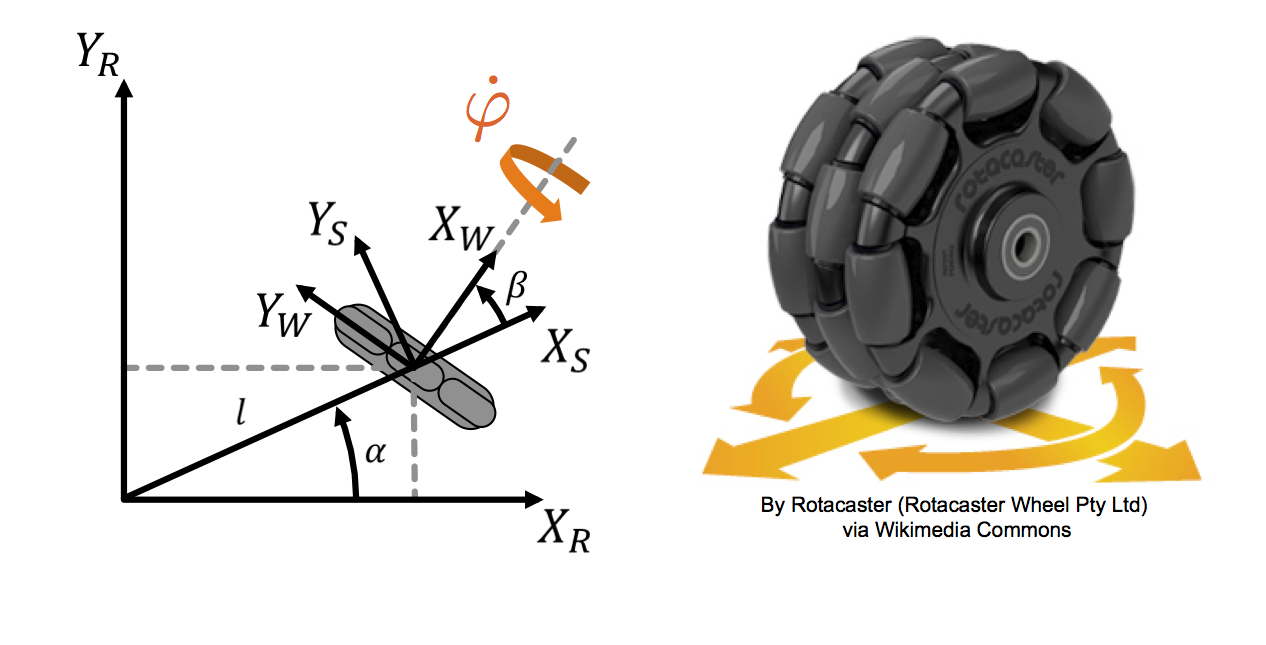
\includegraphics[width=0.8\linewidth]{diagram_2_v100}
\end{figure}
 
\subsection*{Degrees of Freedom}

How many degrees of freedom does this wheel have?

\subsubsection*{Answer}

The answer is 3.

\begin{itemize}
	\item Rotation around the contact point point 
	\item Y axis motion by wheel rotation
	\item X axis motion by Swedish wheel rotation
\end{itemize}

\pagebreak

\subsection*{The Wheel Equation}

Please enter the wheel equation for the 90 degree Swedish wheel pictured above. Pay attention to the turning direction defined in the diagram. This is different than the turning direction defined in the worked example. \\

\noindent In the case of the Swedish wheel, the only actuator/encoder available is the one that spins the large wheel. Movement orthogonal to the large wheel is free due to the rolling of the small wheels. Therefore, the no-sliding-constraint matrix, $\mathbf{C}$, is empty and the wheel equation has the form 

\begin{equation*}
	\mathbf{J} \dot{\xi_R} = r \dot{\varphi}
\end{equation*}

\noindent where $\dot{\xi}_R = [\dot{x} \; \dot{y} \; \dot{\theta}]^T$ is the robot's velocity expressed in the robot frame, r is the radius of the big wheel, and $\dot{\varphi}$ is the turning speed (radians per second) of the big wheel. The matrix $\mathbf{J}$ is $1 \times 3$ and has components 

\begin{equation*}
	\mathbf{J} := [j_1 \quad j_2 \quad j_3]
\end{equation*} \\

\noindent Write an expression for each component of $\mathbf{J}$ in terms of $\alpha$ (alpha), $\beta$ (beta) and $l$ (l). Use the trigonometric functions $\sin$ and $\cos$. Use * for multiplication.

\subsubsection*{Answer}

The constraints of Swedish wheel (with rollers at angle $\gamma$):

\begin{figure}[h]
	\centering
	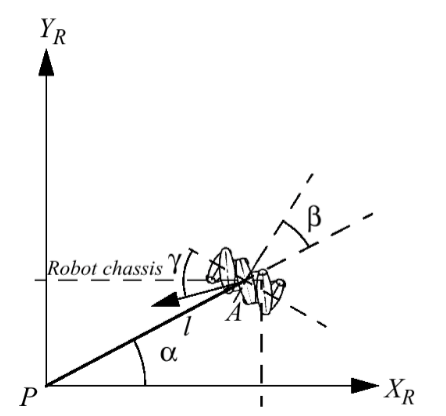
\includegraphics[width=0.5\linewidth]{swedish_wheel}
\end{figure}

\vspace{-5mm}

\begin{align}
	&\begin{bmatrix}
		\sin (\alpha + \beta + \gamma) 	&	- \cos (\alpha + \beta + \gamma) 	&	- l \cos(\beta + \gamma) 
	\end{bmatrix}
	\mathbf{R}(\theta) \dot{\xi}_I - r \dot{\varphi} \cos \gamma = 0 \\ 
	&\begin{bmatrix}
		\cos (\alpha + \beta + \gamma) 	&	\sin (\alpha + \beta + \gamma) 	&	l \sin(\beta + \gamma) 
	\end{bmatrix}
	\mathbf{R}(\theta) \dot{\xi}_I - r \dot{\varphi} \sin \gamma  + r_{sw} \dot{\varphi}_{sw} = 0 
\end{align}

\noindent For 90 degree Swedish wheel, $\gamma = 0$. Thus the rolling constraint equation (1) is as follows:

\begin{equation}
	\begin{bmatrix}
		\sin (\alpha + \beta) 	&	- \cos (\alpha + \beta) 	&	- l \cos(\beta) 
	\end{bmatrix}
	\dot{\xi}_R - r \dot{\varphi} \cos \gamma = 0 
\end{equation} 

\noindent Note that $\mathbf{R}(\theta) \dot{\xi}_I = \dot{\xi}_R$. Therefore,

\begin{align}
	j_1 &= \text{sin (alpha + beta)}\\
	j_2 &= \text{- cos (alpha + beta)}\\
	j_3 &= \text{- l * cos(beta)}
\end{align}

\end{document}